% -*- Mode:TeX -*-

%% IMPORTANT: The official thesis specifications are available at:
%%            http://libraries.mit.edu/archives/thesis-specs/
%%
%%            Please verify your thesis' formatting and copyright
%%            assignment before submission.  If you notice any
%%            discrepancies between these templates and the 
%%            MIT Libraries' specs, please let us know
%%            by e-mailing thesis@mit.edu

%% The documentclass options along with the pagestyle can be used to generate
%% a technical report, a draft copy, or a regular thesis.  You may need to
%% re-specify the pagestyle after you \include  cover.tex.  For more
%% information, see the first few lines of mitthesis.cls. 

%\documentclass[12pt,vi,twoside]{mitthesis}
%%
%%  If you want your thesis copyright to you instead of MIT, use the
%%  ``vi'' option, as above.
%%
%\documentclass[12pt,twoside,leftblank]{mitthesis}
%%
%% If you want blank pages before new chapters to be labelled ``This
%% Page Intentionally Left Blank'', use the ``leftblank'' option, as
%% above. 

\documentclass[12pt,twoside,singlespace]{mitthesis}
\usepackage{lgrind}
%% These have been added at the request of the MIT Libraries, because
%% some PDF conversions mess up the ligatures.  -LB, 1/22/2014
\usepackage{cmap}
\usepackage[T1]{fontenc}
\pagestyle{plain}
\usepackage[sort]{natbib}
%% This bit allows you to either specify only the files which you wish to
%% process, or `all' to process all files which you \include.
%% Krishna Sethuraman (1990).

%\typein [\files]{Enter file names to process, (chap1,chap2 ...), or `all' to
%process all files:}
%\def\all{all}
%\ifx\files\all \typeout{Including all files.} \else \typeout{Including only \files.} \includeonly{\files} \fi

\begin{document}

% -*-latex-*-
% 
% For questions, comments, concerns or complaints:
% thesis@mit.edu
% 
%
% $Log: cover.tex,v $
% Revision 1.8  2008/05/13 15:02:15  jdreed
% Degree month is June, not May.  Added note about prevdegrees.
% Arthur Smith's title updated
%
% Revision 1.7  2001/02/08 18:53:16  boojum
% changed some \newpages to \cleardoublepages
%
% Revision 1.6  1999/10/21 14:49:31  boojum
% changed comment referring to documentstyle
%
% Revision 1.5  1999/10/21 14:39:04  boojum
% *** empty log message ***
%
% Revision 1.4  1997/04/18  17:54:10  othomas
% added page numbers on abstract and cover, and made 1 abstract
% page the default rather than 2.  (anne hunter tells me this
% is the new institute standard.)
%
% Revision 1.4  1997/04/18  17:54:10  othomas
% added page numbers on abstract and cover, and made 1 abstract
% page the default rather than 2.  (anne hunter tells me this
% is the new institute standard.)
%
% Revision 1.3  93/05/17  17:06:29  starflt
% Added acknowledgements section (suggested by tompalka)
% 
% Revision 1.2  92/04/22  13:13:13  epeisach
% Fixes for 1991 course 6 requirements
% Phrase "and to grant others the right to do so" has been added to 
% permission clause
% Second copy of abstract is not counted as separate pages so numbering works
% out
% 
% Revision 1.1  92/04/22  13:08:20  epeisach

% NOTE:
% These templates make an effort to conform to the MIT Thesis specifications,
% however the specifications can change.  We recommend that you verify the
% layout of your title page with your thesis advisor and/or the MIT 
% Libraries before printing your final copy.
\title{Multiscale Methods for Design and Fabrication of Deformable Objects}

\author{Desai Chen}
% If you wish to list your previous degrees on the cover page, use the 
% previous degrees command:
%       \prevdegrees{A.A., Harvard University (1985)}
% You can use the \\ command to list multiple previous degrees
%       \prevdegrees{B.S., University of California (1978) \\
%                    S.M., Massachusetts Institute of Technology (1981)}
\department{Department of Electrical Engineering and Computer Science}

% If the thesis is for two degrees simultaneously, list them both
% separated by \and like this:
% \degree{Doctor of Philosophy \and Master of Science}
\degree{Doctor of Philosophy in Computer Science and Engineering}

% As of the 2007-08 academic year, valid degree months are September, 
% February, or June.  The default is June.
\degreemonth{September}
\degreeyear{2017}
\thesisdate{August 30, 2017}

%% By default, the thesis will be copyrighted to MIT.  If you need to copyright
%% the thesis to yourself, just specify the `vi' documentclass option.  If for
%% some reason you want to exactly specify the copyright notice text, you can
%% use the \copyrightnoticetext command.  
%\copyrightnoticetext{\copyright IBM, 1990.  Do not open till Xmas.}

% If there is more than one supervisor, use the \supervisor command
% once for each.
\supervisor{Wojciech Matusik}{Associate Professor}

% This is the department committee chairman, not the thesis committee
% chairman.  You should replace this with your Department's Committee
% Chairman.
\chairman{Mr. Chairman}{Chairman, Department Committee on Graduate Theses}

% Make the titlepage based on the above information.  If you need
% something special and can't use the standard form, you can specify
% the exact text of the titlepage yourself.  Put it in a titlepage
% environment and leave blank lines where you want vertical space.
% The spaces will be adjusted to fill the entire page.  The dotted
% lines for the signatures are made with the \signature command.
\maketitle

% The abstractpage environment sets up everything on the page except
% the text itself.  The title and other header material are put at the
% top of the page, and the supervisors are listed at the bottom.  A
% new page is begun both before and after.  Of course, an abstract may
% be more than one page itself.  If you need more control over the
% format of the page, you can use the abstract environment, which puts
% the word "Abstract" at the beginning and single spaces its text.

%% You can either \input (*not* \include) your abstract file, or you can put
%% the text of the abstract directly between the \begin{abstractpage} and
%% \end{abstractpage} commands.

% First copy: start a new page, and save the page number.
\cleardoublepage
% Uncomment the next line if you do NOT want a page number on your
% abstract and acknowledgments pages.
% \pagestyle{empty}
\setcounter{savepage}{\thepage}
\begin{abstractpage}
% $Log: abstract.tex,v $
% Revision 1.1  93/05/14  14:56:25  starflt
% Initial revision
% 
% Revision 1.1  90/05/04  10:41:01  lwvanels
% Initial revision
%
%% It will be single-spaced and the rest of the text that is supposed to go on
%% the abstract page will be generated by the abstractpage environment.  This
%% file should be \input (not \include 'd) from cover.tex.
Modern manufacturing technologies such as 3D printing enable the design and fabrication of objects with extraordinary complexity.
Arranging materials to form functional structures can achieve a much wider range of physical properties than in the constituent materials.
Many applications have been demonstrated in the fields of mechanics, acoustics, optics, and electromagnetics.
Unfortunately, it is difficult to design objects manually in the large combinatorial space of possible designs.
Computational design algorithms have been developed to automatically design objects with specified physical properties.
However, many types of physical properties are still very challenging to optimize because predictive and efficient simulations are not available for 
problems such as high-resolution non-linear elasticity or dynamics with friction and impact.
For simpler problems such as linear elasticity, where accurate simulation is available,
the simulation resolution handled by desktop workstations is still orders of magnitudes below available printing resolutions.

We propose to speed up simulation and inverse design process of fabricable objects by using multiscale methods.
First, we construct a library of microstructures and store their material properties such as Young's modulus and Poisson's ratio.
To use the library, the space of achievable material properties called the material property gamut is represented as a level set.
The level set enables efficient sampling of the gamut by focusing on finding samples near and outside the currently sampled boundary.
We use a combination of discrete and continuous sampling methods to push the structures to the limits of achievable material properties.
Next, with a pre-computed gamut, functional objects can be designed using microstructures instead of the base materials.
This allows us to simulate and optimize complex objects at a much coarser scale to improve simulation efficiency.
The speed improvement leads to the designs reaching a trillion voxels to match printer resolutions.
It also enables computational design of dynamic properties that can be faithfully reproduced in reality.
In addition to efficient design optimization, 
the gamut representation of the microstructure envelope provides a way to discover templates of microstructures with extremal physical properties.
In contrast to work where such templates are constructed by hand,
this is the first computational method to automatically discovery microstructure templates from voxel representations.

\end{abstractpage}

% Additional copy: start a new page, and reset the page number.  This way,
% the second copy of the abstract is not counted as separate pages.
% Uncomment the next 6 lines if you need two copies of the abstract
% page.
% \setcounter{page}{\thesavepage}
% \begin{abstractpage}
% % $Log: abstract.tex,v $
% Revision 1.1  93/05/14  14:56:25  starflt
% Initial revision
% 
% Revision 1.1  90/05/04  10:41:01  lwvanels
% Initial revision
%
%% It will be single-spaced and the rest of the text that is supposed to go on
%% the abstract page will be generated by the abstractpage environment.  This
%% file should be \input (not \include 'd) from cover.tex.
Modern manufacturing technologies such as 3D printing enable the design and fabrication of objects with extraordinary complexity.
Arranging materials to form functional structures can achieve a much wider range of physical properties than in the constituent materials.
Many applications have been demonstrated in the fields of mechanics, acoustics, optics, and electromagnetics.
Unfortunately, it is difficult to design objects manually in the large combinatorial space of possible designs.
Computational design algorithms have been developed to automatically design objects with specified physical properties.
However, many types of physical properties are still very challenging to optimize because predictive and efficient simulations are not available for 
problems such as high-resolution non-linear elasticity or dynamics with friction and impact.
For simpler problems such as linear elasticity, where accurate simulation is available,
the simulation resolution handled by desktop workstations is still orders of magnitudes below available printing resolutions.

We propose to speed up simulation and inverse design process of fabricable objects by using multiscale methods.
First, we construct a library of microstructures and store their material properties such as Young's modulus and Poisson's ratio.
To use the library, the space of achievable material properties called the material property gamut is represented as a level set.
The level set enables efficient sampling of the gamut by focusing on finding samples near and outside the currently sampled boundary.
We use a combination of discrete and continuous sampling methods to push the structures to the limits of achievable material properties.
Next, with a pre-computed gamut, functional objects can be designed using microstructures instead of the base materials.
This allows us to simulate and optimize complex objects at a much coarser scale to improve simulation efficiency.
The speed improvement leads to the designs reaching a trillion voxels to match printer resolutions.
It also enables computational design of dynamic properties that can be faithfully reproduced in reality.
In addition to efficient design optimization, 
the gamut representation of the microstructure envelope provides a way to discover templates of microstructures with extremal physical properties.
In contrast to work where such templates are constructed by hand,
this is the first computational method to automatically discovery microstructure templates from voxel representations.

% \end{abstractpage}

\cleardoublepage

\section*{Acknowledgments}

This is the acknowledgements section.  You should replace this with your
own acknowledgements.

%%%%%%%%%%%%%%%%%%%%%%%%%%%%%%%%%%%%%%%%%%%%%%%%%%%%%%%%%%%%%%%%%%%%%%
% -*-latex-*-

% Some departments (e.g. 5) require an additional signature page.  See
% signature.tex for more information and uncomment the following line if
% applicable.
% % -*- Mode:TeX -*-
%
% Some departments (e.g. Chemistry) require an additional cover page
% with signatures of the thesis committee.  Please check with your
% thesis advisor or other appropriate person to determine if such a 
% page is required for your thesis.  
%
% If you choose not to use the "titlepage" environment, a \newpage
% commands, and several \vspace{\fill} commands may be necessary to
% achieve the required spacing.  The \signature command is defined in
% the "mitthesis" class
%
% The following sample appears courtesy of Ben Kaduk <kaduk@mit.edu> and
% was used in his June 2012 doctoral thesis in Chemistry. 

\begin{titlepage}
\begin{large}
This doctoral thesis has been examined by a Committee of the Department
of Chemistry as follows:

\signature{Professor Jianshu Cao}{Chairman, Thesis Committee \\
   Professor of Chemistry}

\signature{Professor Troy Van Voorhis}{Thesis Supervisor \\
   Associate Professor of Chemistry}

\signature{Professor Robert W. Field}{Member, Thesis Committee \\
   Haslam and Dewey Professor of Chemistry}
\end{large}
\end{titlepage}


\pagestyle{plain}
  % -*- Mode:TeX -*-
%% This file simply contains the commands that actually generate the table of
%% contents and lists of figures and tables.  You can omit any or all of
%% these files by simply taking out the appropriate command.  For more
%% information on these files, see appendix C.3.3 of the LaTeX manual. 
\tableofcontents
\newpage
\listoffigures
\newpage
\listoftables


\chapter{Introduction}


\section{Motivations}


\section{Description}\label{ch1:desc}


\subsection{}


\subsection{}

\section{}


\subsection{}

\subsection{}

\section{}

\subsection{}

\subsection{}

\chapter{Data-Driven Coarsening of Finite Elements}
\section{Background}
\subsection{The Finite Element Method}
The finite element method~\citep{ciarlet2002finite} is a way to numerically approximate solutions to partial differential equations.
The function domain $\Omega$ is divided into a finite number of elements $E_k$.
A polynomial function is defined over each element.
These polynomials form a basis for finite-dimensional approximations to the solution.

This thesis uses the eight-node hexahedron element defined in $\mathbb{R}^3$
to perform all of the mechanical analysis.
The eight-node hexahedron element is the simplest of the hexahedron family.
It represents continuous functions supported inside the element by trilinearly interpolating function values defined on its eight nodes.
Each node $\mathbf{X}_i$ resides in $\mathbb{R}^3$ with a given real value $u(\mathbf{X}_i)$.
The nodal positions must cooperate to guarantee that no point inside the hexahedron is inverted.
This will be explained later.
For now, suppose the element shape is well-defined and 
consider a point $\mathbf{X}\in\mathbb{R}^3$ inside the element.
The trilinear interpolation on $\mathbf{X}$ is given by
\[
u(\mathbf{X})=\sum_i N_iu(\mathbf{X}_i),
\]
for some weights $N_i$ that depends on the relative position between $\mathbf{X}$ 
and $\mathbf{X}_i$. These weighting functions are called \textbf{shape functions}.

In order to write down the expression for $N_i$, we need to introduce the standard quadrilateral or hexahedral element (Figure~\ref{fig:standardEle}).
The standard hexahedron is just a cube centered at the origin spanning $[-1,1]^3$.
The axis are labeled with $\xi, \eta, \zeta$ to distinguish from the space that $\mathbf{X}$ resides in.
This new coordinate system is known as the isoparametric hexahedral coordinates or more commonly referred to as \textbf{natural coordinates}.
The nodal positions of the standard elements in the natural coordinates are listed in Table~\ref{tab:natCoord}.
For a point $\chi=(\xi, \eta,\zeta)$ in the natural coordinates,
its interpolation weights is defined as in Equation~\ref{eq:triWeight}.
\begin{equation}
	N_i(\chi)=\frac{1}{8}(1+\xi_i\xi)(1+\eta_i\eta)(1+\zeta_i\zeta).
	\label{eq:triWeight}
\end{equation}
Note that the sum of the weights is always $1$ for any point inside the element.
Suppose now we define a ``density'' value of $1$ on each of its eight vertices,
we can compute the total mass of the element by 
\[
mass=\int_{-1}^{1}\int_{-1}^{1}\int_{-1}^{1}\sum_i w_i\cdot 1 \,d\xi \,d\eta\,d\zeta=
\int_{-1}^{1}\int_{-1}^{1}\int_{-1}^{1} 1 \,d\xi \,d\eta\,d\zeta=8.
\]
This is simply the volume of the standard element multiplied by the density.
This partition of unity property of the interpolation function is crucial for physical meanings of quantities defined on the element.
\begin{figure}
\centering
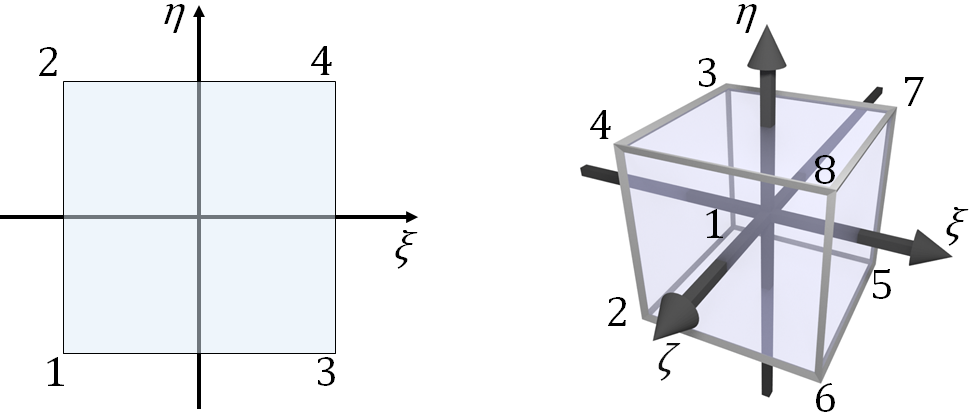
\includegraphics[width=0.8\textwidth]{figs/refEle.png}
\caption{Standard elements for 2D quadrilateral (left) 
	and 3D hexahedral elements (right). The standard element spans $[-1,1]$ in each axis
	to facilitate Gaussian quadrature rules. Nodes are marked with their indices.
	}
\label{fig:standardEle}
\end{figure}
\begin{table}
	\begin{center}
		\begin{tabular}{ |c| r r r|}
			\hline
			Index & $\xi_i$ & $\eta_i$ & $\zeta_i$ \\ \hline
			1 & -1 & -1 & -1\\  
			2 & -1 & -1 & 1\\
			3 & -1 & 1 & -1\\  
			4 & -1 & 1 & 1\\
			5 & 1 & -1 & -1\\  
			6 & 1 & -1 & 1\\
			7 & 1 & 1 & -1\\  
			8 & 1 & 1 & 1\\
		\hline						
		\end{tabular}
	\end{center}
	\caption{Nodal positions of the standard hexahedron element in the natural coordinates.
		Coincidentally, these coordinate values can also be used to define the trilinear interpolation weights.}
	\label{tab:natCoord}
\end{table}

With the interpolation function fully defined in the natural coordinates, 
we can use it to map a point $\chi$ in natural coordinates to a point
$\mathbf{X}$ inside a general hexahedron element with nodal positions $\mathbf{X}_i$ as follows
\begin{equation}
	\mathbf{X}=\sum_i N_i(\chi)\mathbf{X}_i.
	\label{eq:rest}
\end{equation}

Note here we are interpolating a vector-valued function where each coordinate is interpolated independently.
\subsection{Modeling Elastic Objects}
Elastic objects tend to return to its rest shape when deformed by external forces such as stretching, bending, twisting etc. The direction and strength of the tendency to restore to its rest shape is described by its elastic forces.
To model the exact behavior of a small piece of material,
we first use finite elements to approximate its deformations.
A hexahedron element models a piece of elastic material that can deform by changing its nodal positions.
The internal volume deforms by following the nodal displacements using trilinear interpolation.
Of course real materials do not have to deform this way.
The trilinear interpolation is only an approximation.
More precisely, for an element with a rest configuration given by $\mathbf{X}_i$,
its nodes can be moved to new positions $\mathbf{x}_i$ by displacements $\mathbf{u}_i$,
i.e., $\mathbf{x}_i=\mathbf{X}_i+\mathbf{u}_i$.
For any point $\mathbf{X}$ inside the element with known natural coordinates $\chi$, its displacement $\mathbf{u}(\mathbf{X})$ is given by interpolation
\begin{equation}
\mathbf{u}(\mathbf{X}) = \sum_iN_i(\chi)\mathbf{u}_i.
\label{eq:disp}
\end{equation}
To make a clear distinction between $\mathbf{X}$ and $\mathbf{x}$,
$\mathbf{X}$ is defined as a point in the \textbf{reference space} that represents the undeformed shape of an object. The lower case $\mathbf{x}$ lives in the \textbf{deformed space} that represents the deformed configuration of an object.

From now on, to simplify notation, $N_i(\xi)$ will be written as $N_i$.
The deformation of an object is quantified using strain measures,
which is defined in terms of the difference in displacement between nearby points.
Intuitively, if $\mathbf{u}(\mathbf{X})$ is constant, then the displacement field is just a translation. In this case the material is undeformed and should not contain any strain.
More generally, the difference of displacement between nearby points can be written using derivatives,
\[
\mathbf{F}=\frac{\partial \mathbf{u}}{\partial \mathbf{X}}+\mathbf{I}
=\begin{pmatrix}
\dfrac{\partial u_1}{\partial X_1} & \dfrac{\partial u_1}{\partial X_2}&\dfrac{\partial u_1}{\partial X_3}\\
\dfrac{\partial u_2}{\partial X_1} & \dfrac{\partial u_2}{\partial X_2}&\dfrac{\partial u_2}{\partial X_3}\\
\dfrac{\partial u_3}{\partial X_1} & \dfrac{\partial u_3}{\partial X_2}&\dfrac{\partial u_3}{\partial X_3}\\
\end{pmatrix}+\mathbf{I}.
\]
The matrix $\mathbf{F}$ is the \textbf{deformation gradient} and $\mathbf{I}$ is the identity matrix.
While we do not have a closed-form expression of $\mathbf{u}$ written in terms of $\mathbf{X}$,
we have Equation~\ref{eq:rest} and~\ref{eq:disp} that relate $\mathbf{u}$ and $\mathbf{X}$ through $\chi$.
The term $\frac{\partial \mathbf{u}}{\partial \mathbf{X}}$ can be re-written using the chain rule,
\begin{equation}
\frac{\partial \mathbf{u}}{\partial \mathbf{X}}=
\frac{\partial \mathbf{u}}{\partial \chi}
\frac{\partial \chi}{\partial \mathbf{X}}=
(\sum_i\mathbf{u}_i\frac{dN_i}{d\chi})(\frac{\partial \mathbf{X}}{\partial \chi})^{-1}
\label{eq:dudX}
\end{equation}
The matrix $\frac{\partial \mathbf{X}}{\partial \chi}$ is called the Jacobian matrix of $\mathbf{X}$ with respect to $\chi$ and is written as
\[
\mathbf{J}=\frac{\partial \mathbf{X}}{\partial \chi}
= \sum_i\mathbf{X}_i\frac{dN_i}{d\chi}.
\]
By convention, $\frac{dN_i}{d\chi}$ is a $1\times 3$ row vector.
The term $\mathbf{X}_i\frac{dN_i}{d\chi}$ is an outer product that produces a $3\times 3$ matrix.

Given the full expression for the deformation gradient $\mathbf{F}$, we can now define elastic energy densities. 
The elastic energy density function $\Psi(\mathbf{F})$ computes a non-negative energy value given a deformation gradient.
This function fully defines the elastic behavior of a piece of material especially the elastic forces.
Integrating $\Psi$ over the domain $\Omega$ of an element in the reference space yields the total elastic energy contained by that element.
\[
E(\mathbf{x}_1,...,\mathbf{x}_8)=\int_{\Omega}\Psi dV.
\]
Differentiating $E$ with respect to nodal positions $\mathbf{x}_i$ gives us the opposite direction of nodal elastic forces
\[
-\mathbf{f}_i=\frac{dE}{d\mathbf{x}_i}=\int_{\Omega}
\frac{d\Psi(\mathbf{F})}{d\mathbf{F}}
\frac{d\mathbf{F}}{d\mathbf{x}_i}dV
=\int_{\Omega}
\mathbf{P}(\mathbf{F})
\frac{d\mathbf{F}}{d\mathbf{x}_i}dV,
\]
Where
\[
\mathbf{P}(\mathbf{F})=\dfrac{d\Psi(\mathbf{F})}{d\mathbf{F}}.
\]
$\mathbf{P}(\mathbf{F})$ is called the fist Piola-Kirchhoff stress.
It transforms a normal vector in the reference space to a force acting in the deformed configuration divided by area in the reference space.
Integrating in the reference space is not easy since the element is not necessarily a rectangular shape. By change of variables, we can integrate in natural coordinates
in the set $\Omega_{\chi}=[-1,1]^3$.
\begin{align*}
\int_{\Omega}
\mathbf{P}(\mathbf{F})
\frac{d\mathbf{F}}{d\mathbf{x}_i}dV
&=\int_{\Omega_{\chi}}
\mathbf{P}(\mathbf{F})
\frac{d\mathbf{F}}{d\mathbf{x}_i}|\det{\mathbf{J}}|dV\\
&=\int_{\Omega_{\chi}}
\mathbf{P}(\mathbf{F})\mathbf{J}^{-T}
\frac{dN_i}{d\chi}\det{\mathbf{J}}\,dV.
\end{align*}
Here we dropped the absolute value sign because the undeformed element is required to have positive determinant everywhere.
To numerically evaluate the integral, we use Gaussian quadrature rules.
For example, the two-point Gaussian quadrature rule places quadrature points at
$\pm \sqrt{\frac{1}{3}}$ in natural coordinates, which results in $8$ quadrature points with equal weights in 3D.
For each quadrature point $j$, we evaluate the integrand and multiply by the quadrature weight $w_j$. The integral is written as a summation
\[
-\mathbf{f}_i=\sum_j w_j\mathbf{P(\mathbf{F}_j)}\mathbf{J}^{-T}
\frac{dN_i}{d\chi}\det{\mathbf{J}}.
\]

$\Psi$ determines the constitutive model of elasticity, i.e. the relationship between strain measures and stress.
This thesis primarily uses two kinds of constitutive models: linear elasticity and Neo-Hookean model. For the linear elasticity, we first define the infinitesimal strain tensor
\[
\epsilon = \frac{1}{2}(\mathbf{F}+\mathbf{F}^T)-I.
\]
This strain tensor is a symmetric matrix. The stress tensor derived from this strain measure is also a symmetric matrix. This property is a necessary condition for conservation of linear and angular momentum. 
In other words, stress and internal elastic forces should not cause any change in total linear or angular momentum.
The strain energy density function for isotropic linear elasticity is
\[
\Psi(\mathbf{F}) = \mu\epsilon:\epsilon + \frac{\lambda}{2}tr^2(\epsilon).
\]
$\mu$ is a material parameter called shear modulus and $\lambda$ is Lam\'{e}'s first parameter.
$tr(\epsilon)$ is the trace of the strain tensor.
Differentiate $\Psi$ to obtain
\[
\mathbf{P}(\mathbf{F})=\mu(\mathbf{F}+\mathbf{F}^T-2\mathbf{I})+\lambda tr(\mathbf{F}-\mathbf{I})\mathbf{I}.
\]
For anisotropic linear elasticity, the constitutive equation is written as
\begin{equation}
\sigma=\mathbf{C}\epsilon,
\label{eq:constitutive}
\end{equation}
where $\sigma$ is the $3\times 3$ Cauchy stress tensor, $\mathbf{C}$ is a
fourth-order $3\times 3\times3\times3$ tensor called the tensor of elasticity.
The term $\mathbf{C}\epsilon$ is a summation of component-wise products.
In Einstein notation,
\[
\sigma_{ij}=C_{ijkl}\epsilon_{kl}.
\]
Cauchy stress relates to the first Piola-Kirchhoff stress by
\[
\sigma = \frac{1}{\det \mathbf{F}}\mathbf{P}\mathbf{F}^T
\]
The corresponding strain energy density function is
\[
\Psi(\epsilon)=\frac{1}{2}\mathbf{C}\epsilon^2.
\]
To simplify notations, the stress and strain tensors are written as vectors instead of matrices.
Using Voigt notation,
a stress tensor of the form
\[
\sigma=\begin{pmatrix}
\sigma_{xx} & \sigma_{xy} & \sigma_{xz}\\
\sigma_{yx} & \sigma_{yy} & \sigma_{yz}\\
\sigma_{zx} & \sigma_{zy} & \sigma_{zz}
\end{pmatrix}
\]
is rewritten as
\[\sigma=(\sigma_{xx} , \sigma_{yy} , \sigma_{zz},
\sigma_{xy} , \sigma_{yz} , \sigma_{zx}).
\]
This allows the tensor of elasticity to be written as a $6\times 6$ matrix.
For orthotropic linear materials, $\mathbf{C}$ takes the following form
\[
\mathbf{C}=
\begin{pmatrix}
C_{1111} & C_{1122} & C_{1133} & 0 & 0 & 0 \\
 & C_{2222} & C_{2233} & 0 & 0 & 0 \\
& & C_{3333} & 0 & 0 & 0 \\
& & & C_{1212} & 0 & 0 \\
 & Symm &  & & C_{2323} & 0 \\
 & & & & & C_{1313}
\end{pmatrix}.
\]
For a more restricted subset of materials with cubic symmetry, 
$\mathbf{C}$ is specified by three material parameters: Young's modulus $E$,
Poisson's ratio $\nu$, and shear modulus $G$ or $\mu$.
\[\mathbf{C}=
\begin{pmatrix}
(1-\nu)\hat{E} & \nu\hat{E} & \nu\hat{E} & 0 & 0 & 0 \\
&(1-\nu)\hat{E} & \nu\hat{E} & 0 & 0 & 0 \\
& &(1-\nu)\hat{E} & 0 & 0 & 0 \\
& & & \mu & 0 & 0 \\
& Symm &  & & \mu & 0 \\
& & & & & \mu
\end{pmatrix},\hat{E} = \frac{E}{(1-2\nu)(1+\nu)}.
\]

The advantage of the linear elasticity is that it assumes a linear relationship between stress and strain. This leads to a linear relationship between nodal displacements and nodal forces
as follows
\[
\mathbf{K}\mathbf{U}=-\mathbf{f}.
\]
Here $\mathbf{K}$ is called the stiffness matrix given by
\[
\mathbf{K}=\frac{\partial^2 \Psi}{\partial\mathbf{U}^2}.
\]
$\mathbf{U}$ is the concatenated nodal displacement vector
$[\mathbf{u}_1,\mathbf{u}_2,...,\mathbf{u}_8]$ and $\mathbf{f}$ is the concatenated internal nodal force vector.
Computing the deformation under external boundary conditions and forces requires only a single linear solve
\[
\mathbf{U}=\mathbf{K}^{-1}\mathbf{f}_{ext},
\]
given sufficient boundary conditions.
The stiffness matrix is sparse and positive semi-definite (positive definite with enough constraints).
A wide class of linear solvers have been developed for such linear systems.
To see the linear relationship between displacements and force,
we just need to derive the linear relationship between $\epsilon$ and $\mathbf{u}_i$
from Equation~\ref{eq:dudX} and combine it with Equation~\ref{eq:constitutive}.
For a point $\mathbf{X}\in\mathbb{R}^3$, we will use superscripts to denote its individual coordinates.
Define the strain-displacement matrix
\[
\mathbf{B}(\mathbf{X})=
\begin{pmatrix}
\dfrac{dN_1}{d\mathbf{X}^1} & 0 & 0 & ... \\
0 & \dfrac{dN_1}{d\mathbf{X}^2} & 0 & ... \\
0 & 0 & \dfrac{dN_1}{d\mathbf{X}^3} & ... \\
\dfrac{dN_1}{d\mathbf{X}^2} & \dfrac{dN_1}{d\mathbf{X}^1} & 0 & ... \\
0 & \dfrac{dN_1}{d\mathbf{X}^3} & \dfrac{dN_1}{d\mathbf{X}^2} & ... \\
\dfrac{dN_1}{d\mathbf{X}^3} & 0 & \dfrac{dN_1}{d\mathbf{X}^1} & ...
\end{pmatrix}.
\]
For an eight-node hexahedron, this matrix has $3\times 8=24$ columns.
This matrix computes the strain tensor at a point $\mathbf{X}$ given nodal displacements
\[
\epsilon(\mathbf{X})=\mathbf{B}(\mathbf{X})\mathbf{U}.
\]
This linear relationship concludes our claim that linear elasticity model defines a linear relationship between nodal displacements and nodal forces.
Further, using quadrature rules, we can numerically evaluate $\mathbf{K}$ as
\[
\mathbf{K}=\sum_j w_j \mathbf{B}(\mathbf{X}_j)\mathbf{C}\mathbf{B}(\mathbf{X}_j)\det \mathbf{J}.
\]

The downside of linear elasticity is that it does not handle rotation properly.
An elastic object undergoing a rigid rotation should contain zero elastic energy.
If we let $\mathbf{F}=\mathbf{R}$ for some rotation matrix $\mathbf{R}$,
the resulting energy measure is generally non-zero.
This constitutive model is useful only when the deformation is small with respect to the overall size of the object.
When an object undergoes buckling with many potential static equilibrium configurations,
linear elasticity always predict a single solution with little buckling since its elastic energy landscape is convex with a unique local minimum.
Additionally, linear elasticity does not preserve volume according to the Poisson's ratio parameter. In fact, elements can easily invert into non-physical states.

To address the rotation problem, non-linear elasticity models such as the corotated linear elasticity model and the Saint-Venant Kirchhoff model are developed to be rotation invariant.
However, these models still allow an element to invert and do not preserve volume.
We use the Neo-Hookean material model for non-linear elasticity. It resists inverting, and approximately preserves volume according to Poisson's ratio.
The strain energy density of Neo-Hookean model is
\[
\Psi(\mathbf{F})=\frac{\mu}{2}(I_1-3) - \mu \log \det \mathbf{F} 
+ \frac{\lambda}{2}(\log \det \mathbf{F})^2,
\]
where the first isotropic invariant is 
\[
I_1=tr(\mathbf{F}^T\mathbf{F}).
\]
The first Piola-Kirchhoff stress is
\[
\mathbf{P}(\mathbf{F})=\mu(\mathbf{F}-\mathbf{F}^{-T})+\lambda(\log\det\mathbf{F})\mathbf{F}^{-T}.
\]
\section{Data-Driven Coarsening}
Objects with high-resolution, heterogeneous elastic materials are everywhere:
from the output of multimaterial 3D printers to virtual characters 
gracing the screen in our summer blockbusters.
Designing such objects is made possible by the tight coupling of design
tools and numerical simulation which allows designers or automatic
algorithms to update geometry or material parameters and subsequently
estimate the physical effects of the change.
Fast, accurate simulation techniques that can handle runtime changes in geometry
and material composition are a necessity for such iterative design algorithms.
There have been a large number of works on speeding up FEM simulations,
and these speed improvements have enabled FEM to be used in many performance critical tasks 
such as computer animation, surgical training, and virtual/augmented reality.
Even though techniques such as model reduction or numerical coarsening can
achieve order-of-magnitude performance increases,
they require expensive precomputation phases, typically on the order of minutes for large meshes.
This precomputation requires knowledge of an
object’s geometry and material composition a priori, something
that is not known during a design task.
When the user updates the model by changing the geometry or the material distribution,
the preprocessing step must be run again.
As shown in Figure~\ref{fig:typical}a, since this step is inside the design loop,
the user cannot get rapid feedback on the changes made to the object.
\begin{figure}
	\centering
	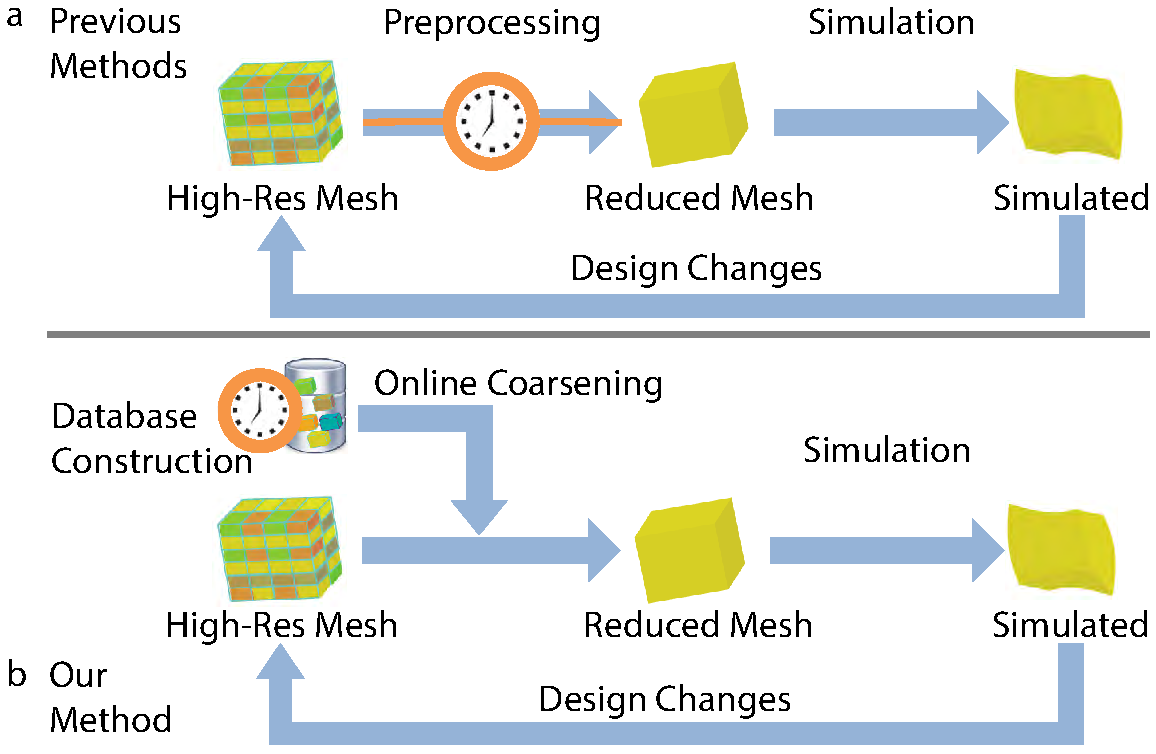
\includegraphics[width=0.8\textwidth]{figs/typical1.pdf}
	\caption{(a) In a typical method, the preprocessing step is offline,
		making the design loop slow. (b) In our method, we move the timeconsuming
		offline computation outside of the design loop.}
	\label{fig:typical}
\end{figure}

We propose Data-Driven FEM (DDFEM), a new simulation methodology
that removes these limitations and is thus extremely well suited
to the types of design problems discussed above.
We divide an object into a set of deformable voxels using embedded finite
elements and coarsen these voxels hierarchically.
A custom metamaterial database is populated with materials that minimize the error incurred by coarsening.
This database is learned once in a completely offline fashion and depends only on the set of materials to be used by the deformable object and not on the actual material distribution
and geometry.
At runtime we use the database to perform fast coarsening of an FEM mesh in a way that is agnostic to changes in geometry and material composition of the object.
The key features of the algorithm are its ability to handle arbitrary, nonlinear elastic
constitutive models as well as to avoid expensive precomputation
within the design loop (Figure~\ref{fig:typical}b).
DDFEM is the first algorithm optimized for interactive design of non-linear elastic objects.

\appendix
\chapter{Code for Using Reduced Templates}
Here we include the Matlab code for generating microstructures given templates and reduced parameters defined in Section~\ref{sec:discovery}.
\lstinputlisting{struct_template.m}
The following function mirrors a microstructure to conform to cubic symmetry.
\lstinputlisting{mirrorCubicStructure.m}
We also include an example input file containing template parameters for Template 5.
The complete microstructure database, templates and reduced parameters are available online~\citep{microDatabase}.
\begin{verbatim}
	5
	0
	54
	0.2 0.24 0.22 0.52 0.47 0.23 
	0.2 0.24 0.25 0.21 0.24 0.09 
	0.45 0.08 0.08 0.28 0.18 0.13 
	0.52 0.23 0.14 0.26 0.2 0.12 
	0.43 0.2 0 0.44 0.18 0.16 
	0.42 0.05 0.06 -0.02 0.01 0.01 
	0.07 0.05 0.02 
	0.05 0.02 -1.13 
	0.08 0.03 0.745 
	0.06 0.01 0.89 
	0.07 0.01 -0.08 
	0.03 0.02 -0.01
	54
	0.207551 0.202924 0.220949 0.565179 0.473398 0.229526 
	0.209012 0.240474 0.250949 0.219012 0.24 0.09 
	0.459051 0.08 0.0899612 0.27 0.179051 0.122411 
	0.519526 0.220474 0.130988 0.27 0.200474 0.12 
	0.43 0.199526 -0.00802498 0.439051 0.18 0.150988 
	0.410513 0.05 0.08 0 0.04 -0.0289737 
	0.0690513 0.0495257 0.0205132 
	0.05 0.02 -1.13 
	0.0804743 0.03 0.744051 
	0.058577 0.01 0.887628 
	0.0695257 0.01 -0.0795257 
	0.03 0.0290125 0.000513167 
	54
	0.184971 0.230649 0.231241 0.51687 0.506269 0.22438 
	0.200296 0.24562 0.261241 0.210296 0.24 0.09 
	0.448759 0.08 0.0915364 0.27 0.168759 0.146565 
	0.51438 0.22562 0.139704 0.27 0.20562 0.12 
	0.43 0.19438 0.00940839 0.428759 0.18 0.159704 
	0.414084 0.05 0.08 0 0.04 -0.0218322 
	0.0587594 0.0443797 0.0240839 
	0.05 0.02 -1.13 
	0.0856203 0.03 0.733759 
	0.0431392 0.01 0.861899 
	0.0643797 0.01 -0.0743797 
	0.03 0.0202958 0.00408392 
	54
	0.2 0.24 0.22 0.52 0.47 0.23 
	0.2 0.24 0.25 0.21 0.24 0.08 
	0.46 0.08 0.08 0.29 0.18 0.13 
	0.52 0.23 0.14 0.26 0.2 0.12 
	0.43 0.19 0.01 0.44 0.18 0.16 
	0.43 0.06 0.04 0 0 0 
	0.07 0.05 0.02 
	0.05 0.02 -1.13 
	0.06 0.03 0.745 
	0.05 0.01 0.89 
	0.07 0.01 -0.08 
	0.04 0.02 0
	54
	0.19 0.22 0.22 0.55 0.49 0.23 
	0.2 0.24 0.25 0.21 0.24 0.09 
	0.46 0.08 0.08 0.27 0.18 0.13 
	0.51 0.22 0.14 0.27 0.2 0.12 
	0.43 0.2 0 0.44 0.18 0.16 
	0.42 0.05 0.08 0 0.04 -0.03
	0.07 0.05 0.03 
	0.05 0.02 -1.13 
	0.08 0.03 0.745 
	0.06 0.01 0.89 
	0.07 0.01 -0.08 
	0.03 0.02 0	
\end{verbatim}
\chapter{Figures}

\vspace*{-3in}

\begin{figure}
\vspace{2.4in}
\caption{Armadillo slaying lawyer.}
\label{arm:fig1}
\end{figure}
\clearpage
\newpage

\begin{figure}
\vspace{2.4in}
\caption{Armadillo eradicating national debt.}
\label{arm:fig2}
\end{figure}
\clearpage
\newpage

%% This defines the bibliography file (main.bib) and the bibliography style.
%% If you want to create a bibliography file by hand, change the contents of
%% this file to a `thebibliography' environment.  For more information 
%% see section 4.3 of the LaTeX manual.
\begin{singlespace}
\bibliography{main}
\bibliographystyle{plainnat}
\end{singlespace}

\end{document}

